\documentclass[12pt]{article}
\usepackage{amsmath}
\usepackage{float}
\usepackage{algorithm}
\usepackage{amssymb}
\usepackage{graphicx}
\usepackage{hyperref}
\usepackage{cleveref}
\usepackage[most]{tcolorbox}
\usepackage[utf8]{inputenc}
\usepackage{tikz}
\usepackage{pstricks-add}
\usepackage{centernot}
\usepackage{algpseudocode}
\usepackage{enumerate}
\usepackage{MnSymbol}
\usepackage{mathtools}
\usepackage{subcaption}
\usepackage{geometry}
 \geometry{
 a4paper,
 total={170mm,257mm},
 left=20mm,
 top=20mm,
 }
\DeclarePairedDelimiter\ceil{\lceil}{\rceil}
\DeclarePairedDelimiter\floor{\lfloor}{\rfloor}
\DeclarePairedDelimiter\abs{\left|}{\right|}
\DeclareMathOperator{\arcsec}{arcsec}
\DeclareMathOperator{\arccot}{arccot}
\DeclareMathOperator{\arccsc}{arccsc}
\hypersetup{
    colorlinks=false,
    pdfborder={0 0 0},
}
\newcommand\tab[1][1cm]{\hspace*{#1}}
\newtheorem{theorem}{Theorem}
\newtheorem{corollary}{Corollary}
\usetikzlibrary{arrows,calc}
\title{MAT 1001: Calculus I}
\author{Alfonsus Rodriques Rendy}
\date{2021-11-22}

\begin{document}
\begin{center}
    \hspace*{-0.5cm}
    \framebox{
    \begin{minipage}{1\linewidth}
        \textbf{MAT1001 Calculus I} \\
        \vspace{-0.8cm}
        \begin{center}
            \huge{Lecture 21 - 25 : Techniques of Integration} 
            \\
            \vspace{0.5cm}
            \normalsize \textit{Lecture by Dr. Arjan Abeynaike} \\
            \vspace{0.3cm}
            \text{Scribe by Alfonsus Rodriques Rendy} \\
            \textrm{Nov 22, 2021 - Dec 7, 2021}
        \end{center}
    \end{minipage}}
\end{center}

\section{Integration by Parts}
\subsection{Integration by Parts}
Integration by parts is a technique that simplifies integrals. If $f$ and $g$ are differentiable at $x$, then 
\[
    (f(x)g(x))' = f'(x)g(x) + f(x)g'(x)
\]
\paragraph{Formula} Integration by Parts
\[
    \int f(x)g'(x) \, dx = f(x)g(x) - \int f'(x)g(x) \, dx
\]
or if we consider $u = f(x)$ and $v = g(x)$ then it can be written as
\[
    \int u\, dv = uv - \int v \, du
\]

\paragraph{Example 1} $\int x \cos x \, dx$
\begin{align*} 
    \int x \cos x \, dx &= x \sin x - \int \sin x \, dx \\
    &= x \sin x + \cos x + C
\end{align*}

\paragraph{Example 2} $\int x^2 e^x \, dx$
\begin{align*} 
    \int x^2 e^x \, dx &= x^2 e^x - \int 2x e^x \, dx \\
    &= x^2 e^x - (2x e^x - \int 2 e^x \, dx) \\
    &= x^2 e^x - 2xe^x + 2e^x + C
\end{align*}

\paragraph{Example 3} $\int e^x \sin x \, dx$
\begin{align*} 
    \int e^x \sin x \, dx &= - e^x \cos x + \int e^x \cos x \, dx \\
    &= -e^x \cos x + e^x \sin x - \int e^x \sin x \\
    2 \int e^x \sin x &= e^x (\sin x - \cos x) + C_1 \\
    \int e^x \sin x &= \frac{1}{2} e^x (\sin x - \cos x) + C\\
\end{align*}

\subsection{Reduction Formulae}
Consider finding $I = \int \sin^n x \, dx$ where $n \neq 0$
Set $u = \sin^{n-1} x$ and $dv = \sin x dx$ then $I = \int u \, dv$
Then 
\[
    du = (n - 1) \sin^{n - 2} x (\cos x) \, dx 
\]
\[
    v = - \cos x
\]

\begin{align*} 
    I &= \int \sin^n x \, dx = uv - \int v \, du \\
    &= (\sin^{n - 1} x)( - \cos x) - \int ( - \cos x)(n - 1)\sin^{n - 2} (\cos x) \, dx \\
    &= - \sin^{n - 1} x \cos x + (n - 1) \int \sin^{n - 2} x \cdot \cos^2 x \, dx \\
    &= - \sin^{n - 1} x \cos x + (n - 1) \int \sin^{n - 2} x \cdot (1 - \sin^2 x)\, dx \\
    &= - \sin^{n - 1} x \cos x + (n - 1) \int \sin^{n - 2} x \, dx - (n - 1) \int \sin^{n} x \, dx \\
    I &= - \sin^{n - 1} x \cos x + (n - 1) \int \sin^{n - 2} x \, dx - (n - 1)I \\
    nI &= - \sin^{n - 1} x \cos x + (n - 1) \int \sin^{n - 2} x \, dx \\
    I &= - \frac{1}{n} \sin^{n - 1} x \cos x\, + \frac{n - 1}{n} \int \sin^{n - 2} x \, dx
\end{align*}

\paragraph{Reduction Formulae}
\[
    \int \sin^n x \, dx = - \frac{1}{n} \sin^{n - 1} x \cos x\, + \frac{n - 1}{n} \int \sin^{n - 2} x \, dx \\
\]
\[
    \int \cos^n x \, dx = \frac{1}{n}\cos^{n - 1} x  \sin x\, + \frac{n - 1}{n} \int \cos^{n - 2} x \, dx \\
\]

\paragraph{Example} Evaluate $\int \sin^3 x \, dx$
\begin{align*} 
    \int \sin^3 x &= -\frac{1}{3} \cos x \sin^2 x + \frac{2}{3} \int \sin x \, dx \\
    &= - \frac{1}{3} \cos x \sin^2 x - \frac{2}{3} \cos x + C
\end{align*}

\paragraph{Reduction Formulae for $\tan x$} 
\[
    \int \tan^m x \, dx \textrm{\tab} (m \in \mathbb{N})
\]
Assume $m \geq 2$ then 
\begin{align*} 
    \int \tan^m x \, dx &= \int (\tan^{m - 2} x)(\tan^2 x) \, dx \\
    &= \int (\tan^{m - 2})(\sec^2 x - 1) \, dx \\
    &= \int (\tan^{m - 2})(\sec^2 x) \, dx -  \int (\tan^{m - 2}) \, dx
\end{align*}
Let $u = \tan x$
\begin{align*} 
    \int (\tan^{m - 2})(\sec^2 x) \, dx - \int (\tan^{m - 2}) \, dx &= \int u^{m - 2} \, du - \int (\tan^{m - 2}) \, dx \\
    &= \frac{u^{m - 1}}{m - 1} - \int (\tan^{m - 2}) x \, dx \\
    &= \frac{\tan^{m - 1} x}{m - 1} - \int (\tan^{m - 2} x) \, dx \\ 
\end{align*}

\paragraph{Reduction Formulae for $\sec x$} 
\[
    \int \sec^n x \, dx \textrm{\tab} (n \in \mathbb{N})
\]
Assume $n \geq 3$, Let $u = \sec^{n - 2} x$ and $dv = \sec^2 x dx$
\begin{align*} 
    \int \sec^n x \, dx &= \sec^{n - 2} x \cdot \tan x - (n - 2)\int(\sec^{n - 2} x)(\tan^2 x) \, dx \\
    &= \sec^{n - 2} x \cdot \tan x - (n - 2)\int(\sec^{n - 2} x)(\sec^{n - 2} x - 1) \, dx \\
    &= \sec^{n - 2} x \cdot \tan x - (n - 2)\int(\sec^{n} x) \, dx + (n - 2)\int(\sec^{n - 2} x) \, dx \\
    (n - 1)\int \sec^n x \, dx &=  \sec^{n - 2} x \cdot \tan x + (n - 2)\int(\sec^{n - 2} x) \, dx \\
    \int \sec^n x \, dx &= \frac{\sec^{n - 2} x \cdot \tan x}{n - 1}  + \frac{n - 2}{n- 1} \int(\sec^{n - 2} x) \, dx \\
\end{align*}

\subsection{Definite Integrals by Parts}
If $f'(x)g(x) + f(x)g'(x)$ is continuous on $[a, b]$ then by FTC2:
\[
    \int_a^b f'(x)g(x) + f(x)g'(x) = f(x)g(x) |_a^b 
\]
Hence 
\[
    \int_a^b f(x)g'(x) = f(x)g(x) |_a^b - \int_a^b f'(x)g(x) \, dx
\]

\paragraph{Example} Evaluate $\int_0^1 \arctan x \, dx$ \\
Let $u = \arctan x$ and $dv = dx$
\begin{align*} 
    \int_0^1 \arctan x \, dx &= x\arctan x \mid_0^1 - \int_0^1 \frac{x}{1 + x^2} \, dx \\
    &= \arctan 1 - \left[ \frac{1}{2} \ln (1 + x^2) \right]_0^1 \\
    &= \frac{\pi}{4} - \frac{1}{2}\ln 2
\end{align*}
    
\subsection{Tabular Integration}
Consider finding $\int x^{10} \cos x \, dx$. We can apply integration by parts 10 times or simply use tabular integration.
Now suppose we have
\[
    g'_i (x) = g_{i - 1}(x)
\]
So, upon integrating we can get
\[
    g(x) = g_0(x) \to g_1(x) \to g_2(x) \to \dots  \to g_m(x)
\]
Then 
\begin{align*} 
    \int f_0(x)g_0(x) \, dx &= f_0(x)g_1(x) - \int f_1(x)g_1(x) \, dx \\
    &= f_0(x)g_1(x) - f_1(x)g_2(x) + \int f_2(x)g_2(x) \, dx \\
    &= \dots \\
    &= f_0(x)g_1(x) - f_1(x)g_2(x) + f_2(x)g_3(x) - \dots \pm \int f_m(x)g_m(x) \, dx
\end{align*}
This method is particularly effective for solving $\int x^n g(x) \, dx$

\section{Integral of Trigonometric Functions}
\subsection{Power of $\sin x$ and $\cos x$}
\[
    \int \sin^m \cos^n \, dx\, \textrm{\tab} (m, n \in \mathbb{N})
\]
\noindent
(1) If $m$ or $n$ is odd, consider one of them and take out all the even powers.
(e.g. $m = 5$ then write $\sin^5 x = (\sin^2 x)^2 \sin x$) and use $\sin^2 x + \cos^2 x = 1$.

\paragraph{Example 1} Evaluate $\int \sin^5 x \cos^7 x \, dx$
\begin{align*} 
    \int \sin^5 \cos^7 x \, dx &= \int (\sin^2 x)^2 \sin x \cos^7 x \, dx \\
    &= \int (1 -\cos^2 x)^2 \sin x \cos^7 x \, dx \\
\end{align*}
Let $u = \cos x$ then $dx = du/(-\sin x)$
\begin{align*} 
    \int (1 -\cos^2 x)^2 \sin x \cos^7 x \, dx &= - \int (1 - u^2)^2 u^7 \, du \\
    &= -\int u^7 (1 - 2u^2 + u^4) \, du \\
    &= - \int u^7 - 2u^9 + u^{11} \, du \\
    &= - \frac{1}{8}u^8 + \frac{1}{5} u^{10} - \frac{1}{12} u^{12} + C \\
    &= - \frac{1}{8} \cos^8 x + \frac{1}{5} \cos^{10} x - \frac{1}{12} \cos^{12} x + C \\
\end{align*}
\paragraph{Example 2} Evaluate $\int cos^7 x \, dx $
\begin{align*} 
    \int \cos^7 x \, dx &= \int (\cos^2x)^2 \cos x dx \\
    &= \int (1 - \sin^2x)^3 \cos x \, dx \\
    &= \int (1 - u^2)^3 \, du \\
    &= \int 1 - 3u^2 + 3u^4 - u^6 \, du \\
    &= u - u^3 + \frac{3}{5} u^5 - \frac{1}{7} u^7 + C \\
    &= \sin x - \sin^3 x + \frac{3}{5} \sin^5 x - \frac{1}{7} \sin^7 x + C
\end{align*}

\noindent
(2) If both $m$ and $n$ is even, then use half angle identities:
\[
    \sin^2 = \frac{1 - \cos 2x}{2} \textrm{\tab or \tab} \cos^2 x = \frac{1 + \cos 2x}{2} 
\]

\paragraph{Example} Evaluate $\int \sin^2 x \cos^4 x \, dx$
\begin{align*} 
    \int \sin^2 x \cos^4 x \, dx &= \int \sin^2 x(\cos^2 x)^2 \, dx \\
    &= \int \left( \frac{1 - \cos 2x}{2}  \right) \left( \frac{1 + \cos 2x}{2} \right)^2 \, dx \\
    &= \frac{1}{8} \int (1 + \cos 2x - \cos^2 2x - \cos^3 2x) \, dx \\
\end{align*}

\[
    \int (1 + \cos 2x) \, dx = x + \frac{1}{2} \sin 2x + C_1
\]
\[
    \int \cos^2 2x \, dx = \int \frac{1 + \cos 4x}{2} \, dx = \frac{1}{2}x + \frac{1}{8} \sin 4x + C_2 
\]
\begin{align*} 
    \int \cos^3 2x \, dx &= \int (1 - \sin^2 2x) \cos 2x \, dx \\
    &= \int (1 - u^2) \frac{1}{2} \, du \\
    &= \frac{1}{2} (u - \frac{1}{3}u^3) + C_3 \\
    &= \frac{1}{2} \left( \sin 2x - \frac{1}{3} \sin^3 2x \right) + C_3
\end{align*}

\[
    \int \sin^2 x \cos^4 x \, dx = \frac{1}{8} \left( \frac{1}{2}x - \frac{1}{8} \sin 4x + \frac{1}{6} \sin^3 2x \right) + C
\]

\subsection{Power of $\tan x$ and $\sec x$}
\[
    \tan^m x \sec^n x \, dx \textrm{\tab} (m, n \in \mathbb{Z}_{+})
\]
(1) If $n$ is even then take out a copy of $\sec^2 x$ and express everything in terms of $\tan x$
\begin{align*} 
    \int (\tan^m x)(\sec^{2k} x) \, dx &= \int (\tan^m x)(\sec^{2k - 2} x)(\sec^2 x) \, dx \\
    &= \int \tan^m x (1 + \tan^2 x)^{k - 1} d(\tan x)
\end{align*}

\noindent
(2) If $n$ is odd and $m$ is odd, then take out a copy of $\tan x \sec x$ and express the rest in terms of $\sec x$
\begin{align*} 
     \int (\tan^{2r + 1} x)(\sec^{2k + 1} x) \, dx &= \int (\tan^{2r} x)(\sec^{2k} x)(\tan x \sec x) \, dx \\ 
     &= \int (\sec^2 x - 1)^r (\sec^{2k} x) d(\sec x)
\end{align*}

\noindent
(3) If $m$ is even, then use $\tan^2 x = \sec^2 x - 1$ and convert the integrand into sums of powers of $\sec x$
\begin{align*} 
    \int (\tan^{2r} x)(\sec^n ) \, dx = \int (\sec^2 x - 1)^r (\sec^n x) \, dx
\end{align*}
Then use the reduction formula for $\int \sec^t x \, dx$

\subsection{Integrals with Square Roots}
For integrals with square roots, trigonometry identities involving squares may help remove square roots signs. 
\[
    \sin^2 x = \frac{1 - \cos 2x}{2} \textrm{\tab or \tab} \cos^2 x = \frac{1 + \cos 2x}{2} 
\]
\paragraph{Example} Evaluate
\[
    \int_0^{\frac{\pi}{4}} \sqrt{1 + \cos 4x} \, dx 
\]

\begin{align*} 
    \int_0^{\frac{\pi}{4}} \sqrt{1 + \cos 4x} \, dx &= \int_0^{\frac{\pi}{4}} \sqrt{2 \cos^2 2x}\\
    &= \sqrt{2} \int_0^{\frac{\pi}{4}} \cos 2x \, dx \\
    &= \frac{\sqrt{2}}{2} \sin 2x \mid_0^{\frac{\pi}{4}} \\
    &= \frac{\sqrt{2}}{2}
\end{align*}

\subsection{Product of Sine and Cosine Functions}
\begin{align*} 
    \sin mx \sin nx = \frac{1}{2} [\cos (m - n)x - \cos(m + n)x] \\
    \sin mx \cos nx = \frac{1}{2} [\sin (m - n)x + \sin(m + n)x] \\
    \cos mx \cos nx = \frac{1}{2} [\cos (m - n)x + \cos(m + n)x]
\end{align*}

\paragraph{Example} Evaluate 
\[
    \int \sin 4x \cdot \cos 8x \, dx
\]
\begin{align*} 
    \int \sin 4x \cdot \cos 8x \, dx &= \int \frac{1}{2} \sin ( - 4x) + \frac{1}{2} \sin (12x) \, dx \\
    &= \frac{1}{2} \int \sin( - 4x) \, dx + \frac{1}{2} \int \sin(12x) \, dx
\end{align*}
\section{Trigonometric Substitution}
Trigonometric substitutions can be useful when integrating functions involving $\sqrt{a^2 - x^2}$, $\sqrt{x^2 - a^2}$, or $\sqrt{a^2 + x^2}$.
We use the following identities:
\begin{itemize} 
    \item $1 - \sin^2 x = \cos^2 x$ for $\sqrt{a^2 - x^2}$ and use substitution $x = a\sin x$
    \item $\sec^2 x - 1 = \tan^2 x$ for $\sqrt{x^2 - a^2}$ and use substitution $x = a\sec x$
    \item $1 + \tan^2 x = \sec^2 x$ for $\sqrt{a^2 + x^2}$ and use substitution $x = a\tan x$
\end{itemize}
\begin{figure}[H]
     \centering
     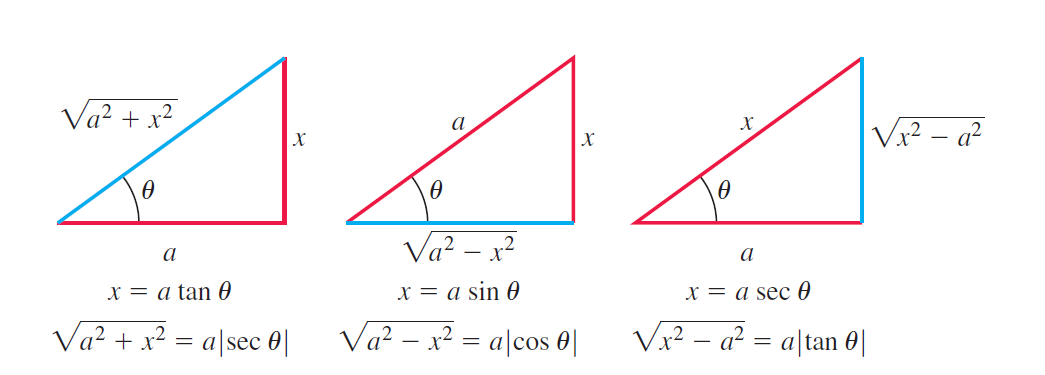
\includegraphics[width = 0.7 \linewidth]{Images/trig substitution.png}
     \caption{Triangle reference of trigonometry substitution}
\end{figure}

\paragraph{Example 1} Evaluate
\[
    \int \frac{dx}{\sqrt{9 + x^2}} 
\]
Let $x = 3 \tan \theta$, $\frac{-\pi}{2} < \theta < \frac{\pi}{2}$
\begin{align*} 
    \int \frac{dx}{\sqrt{9 + x^2}}\, &= \int \frac{3 \sec^2 \theta d\theta}{\sqrt{9 + 9 \tan^2 \theta}} \\
    &= \int \frac{3 \sec^2 \theta d\theta}{3\sqrt{1 + 1 \tan^2 \theta}} \\
    &= \int \frac{3 \sec^2 \theta d\theta}{\sqrt{3\sec^2 \theta}} \\
    &= \int \sec \theta\, d\theta \\
    &= \ln \mid \sec \theta + \tan \theta \mid + C \\
    &= \ln \left| \frac{\sqrt{9 + x^2}}{3} + \frac{x}{3} \right| + C 
\end{align*}

\paragraph{Note} For the substitution $x = f(\theta)$, the domain of $f$ is chosen so that $f$ is injective (one-to-one) and covers all the possible values of $x$.
We choose the standard domains of thoe trigonometric functions.

\paragraph{Example 2} Evaluate 
\[
    \int \frac{dx}{x^2 \sqrt{x^2 - 4}} 
\]
Let $x = 2\sec \theta$, then $dx = 2\sec \theta \tan \theta \, d\theta$

\begin{align*} 
    \int \frac{dx}{x^2 \sqrt{x^2 - 4}} &= \int \frac{2 \sec \theta \tan \theta \, d\theta}{4 \sec^2 \theta \cdot 2 \sqrt{\tan^2 \theta}} \\
    &= \frac{1}{4} \int \frac{\tan \theta d\theta}{\sec \theta \cdot | \tan \theta |} \\
    &= \begin{cases}\, 
        \frac{1}{4} \sin \theta \, d\theta & x > 2 \\
        - \frac{1}{4} \sin \theta \, d\theta & x < - 2 
    \end{cases}\, 
\end{align*}
Since 
\[
    \sin \theta\, = \sqrt{1 - \cos^2 \theta} = \sqrt{1 - \frac{1}{\sec^2 \theta}} = \sqrt{\frac{x^2 - 4}{x^2}} = \begin{cases} 
        \frac{1}{x} \sqrt{x^2 - 4} & x > 2 \\
        - \frac{1}{x} \sqrt{x^2 - 4} & x < - 2
    \end{cases} 
\]
So,
\[
    \int \frac{dx}{x^2 \sqrt{x^2 - 4}} = \frac{1}{4x} \sqrt{x^2 - 4}
\]
\paragraph{Example 3} Find the area of the ellipse 
\[
    \frac{x^2}{a^2} + \frac{y^2}{b^2} = 1 
\]
\begin{figure}[H]
     \centering
     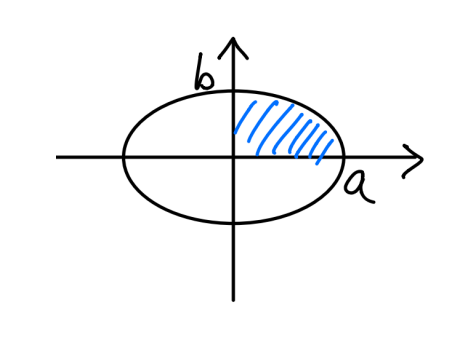
\includegraphics[width = 0.4 \linewidth]{Images/ellipse area.png}
\end{figure}
Let area $A = 4A_1$, where $A_1$ is the shaded area.
\[
    \frac{x^2}{a^2} + \frac{y^2}{b^2} = 1 \Leftrightarrow y^2 = b^2 (1 - \frac{x^2}{a^2} ) = \frac{b^2}{a^2}(a^2 - x^2) 
\]
Hence, 
\[
    y = \frac{b}{a} \sqrt{a^2 - x^2} \textrm{\tab for } y > 0
\]

Let $x = a\sin \theta$
\begin{align*} 
    A_1 = \frac{b}{a} \int_0^a \sqrt{a^2 - x^2} \, dx\, 
    &= \frac{b}{a} \int_0^{\frac{\pi}{2}} \sqrt{a^2 - a^2 \sin^2 \theta}\, d\theta\ \\
    &= ab \int_0^{\frac{\pi}{2}} \cos^2 \theta d\theta \\
    &= ab \int_0^{\frac{\pi}{2}} \frac{1 + \cos 2\theta}{2} d\theta \\
    &= \frac{ab}{2} \left[ \theta + \frac{1}{2} \sin 2 \theta \right]_0^{\frac{\pi}{2}} \\
    &= \frac{ab\pi}{4}
\end{align*}
    
\[
    A = 4A_1 = ab\pi 
\]
\section{Integral by Partial Fractions}
\subsection{Partial Fractions}
\paragraph{Definition} If $P(x) = a_nx^n + a_{n-1}x^{n-1} + ... + a_1x + a_0$ with $a_n \neq 0$,
then deg($P(x)$) = $n$, deg($P(x)$) is called the degree of $P(x)$

\paragraph{Example} deg($7x^3 - 2x^2 + \pi x + e$) = 3 and deg($a_0$) = 0

If deg($P(x)$) $\geq$ deg($Q(x)$) then by long division, we can find polynomials $S(x)$ and $R(x)$ such that
\[
    \frac{P(x)}{Q(x)} = S(x) + \frac{R(x)}{Q(x)} 
\]
with deg($R(x)$) $<$ deg($Q(x)$).

Every polynomial factors into linear or irreducible quadratic polynomials over the real numbers. A quadratic polynomial $ax^2 + bx + c$ is irreducible 
if it has no real root, i.e., if $b^2 - 4ac < 0$. Then, every non-zero polynomial $Q(x)$ can be written as 
\[
    Q_1(x)Q_2(x)\dots Q_k(x)
\]
where each $Q_i(x)$ is either linear $a_i x + b_i, a_i \neq 0$ or irreducible quadratic polynomials with the form of $a_i x^2 + b_i x + c_i, a_i \neq 0, b_i^2 - 4a_ic_i < 0$.

\paragraph{Example} $x^2 - 1$ = $(x - 1)(x + 1)$ meanwhile $x^2 + 1$ is irreducible in $\mathbb{R}$ ($x^2 + 1$ is still reducible in $\mathbb{C}$ with the factor $(x + i)(x-i), i = \sqrt{-1}$).
$x^4 + 1 = (x^2 + \sqrt{2}x + 1)(x^2 - \sqrt{2}x + 1)$

\paragraph{Example of Long Division} 
\[
    \frac{x^3 - 4x^2 + 2x - 3}{x + 2} = x^2 - 6x + 14 - \frac{31}{x + 2} 
\]
then
\begin{align*} 
    \int \frac{x^3 - 4x^2 + 2x - 3}{x + 2} dx &= \int x^2 - 6x + 14 dx - 31\int \frac{1}{x + 2} dx \\
    &= \frac{1}{3} x^3 - 3x^2 + 14x - 31 \ln |x + 2| + C
\end{align*}

\paragraph{Finding Partial Fractions}
Now we focus on $\frac{P(x)}{Q(x)}$ with deg($P(x)$) $<$ deg($Q(x)$).

\paragraph{Case 1} $Q(x)$ is a product of distinct linear factors:
\[
    Q(x) = (a_1x + b_1)(a_2x + b_2)\dots (a_kx + b_k)
\]
In this case, there exists constants $A_1, A_2, ... A_k$ such that
\[
    \frac{P(x)}{Q(x)} = \frac{A_1}{a_1x + b_1} + \frac{A_2}{a_2x + b_2} + \dots + \frac{A_k}{a_kx + b_k} 
\]

\paragraph{Example Case 1} Find
\[
    \int\,\frac{x^2 + 2x - 1}{2x^3 + 3x^2 - 2x}\, dx 
\]

(1) Find the factors of the denominator:
\[
    2x^3 + 3x^2 - 2x = x(2x - 1)(x + 2)
\]

(2) Split the fraction up, keeping $A, B, C$ as undetermined coefficients
\[
    \frac{x^2 + 2x - 1}{2x^3 + 3x^2 - 2x} = \frac{A}{x} + \frac{B}{2x - 1} + \frac{C}{x + 2}
\]

then 
\[
    x^2 + 2x - 1 = A(2x - 1)(x + 2) + Bx(x + 2) + Cx(2x - 1)
\]

(3) Find the coefficients $A, B, C$
\[
    x^2 + 2x - 1 = (2A + B + 2C)x^2 + (3A + 2B - C)x - 2A
\]
\begin{align*} 
     2A + B + 2C &= 1 \\
     3A + 2B - C &= 2 \\
     - 2A &= - 1
\end{align*}
We can find that $A = \frac{1}{2}$, $B = \frac{1}{5}$ and $C = \frac{-1}{10}$
Hence we have
\begin{align*} 
    \frac{x^2 + 2x - 1}{2x^3 + 3x^2 - 2x} \, dx &= \int \frac{1}{2} \frac{1}{x} \, dx + \int \frac{1}{5} \frac{1}{2x - 1} \, dx - \int \frac{1}{10} \frac{1}{x + 2} \, dx \\
    &= \frac{1}{2} \ln |x| + \frac{1}{10} \ln |2x - 1| - \frac{1}{10} \ln|x + 2| + C
\end{align*}
\paragraph{Case 2} $Q(x)$ is a product of linear factors, some of which are repeated \\ \\
Suppose that a linear factor $a_1x + b_1$ is repeated $r$ times, that is $(a_1x + b_1)^r$ appears in the factorization of $Q(x)$. Then instead of just taking the single term of $\frac{A_1}{a_1x + b_1}$, we would use
\[
    \frac{A_1}{a_1x + b_1} + \frac{A_2}{(a_1x + b_1)^2} + \dots\, + \frac{A_r}{(a_1x + b_1)^r} 
\]

\paragraph{Example Case 2} Find
\[
    \int \frac{x^4 - 2x^2 + 4x + 1}{x^3 - x^2 - x + 1} \, dx 
\]

(1) Applying long division to get the remainder 
\[
    \frac{x^4 - 2x^2 + 4x + 1}{x^3 - x^2 - x + 1} = x + 1 + \frac{4x}{x^3 - x^2 - x + 1} 
\]

(2) Factorize the denominator $\frac{4x}{x^3 - x^2 - x + 1}$
\[
    x^3 - x^2 - x + 1 = x^2(x - 1) - (x - 1) = (x + 1)(x -1)^2
\]

(3) Split up the fraction 
\[
    \frac{x^4 - 2x^2 + 4x + 1}{x^3 - x^2 - x + 1} = \frac{A}{x - 1} + \frac{B}{(x - 1)^2} + \frac{C}{x + 1}
\]

Then
\[
    4x = A(x - 1)(x + 1) + B(x + 1) + C(x - 1)^2
\]

(4) Find the coefficients $A, B, C$
\[
    4x = (A + C)x^2 + (B - 2C)x + ( - A + B + C)
\]

\begin{align*} 
     A + C &= 0 \\
     B - 2C &= 4 \\
     - A + B + C &= 0 
\end{align*}
We can find that $A = 1$, $B = 2$, $C = -1$.

(5) Solve the integral of the partial Fractions
\begin{align*} 
    \int \frac{x^4 - 2x^2 + 4x + 1}{x^3 - x^2 - x + 1} \, dx &= \int (x + 1) \, dx + \int \frac{4x}{x^3 - x^2 - x + 1} \\ 
    &= \frac{1}{2}x^2 + x + \int \frac{dx}{x - 1} + \frac{2dx}{(x - 1)^2} - \frac{dx}{x + 1} + C_1 \\
    &= \frac{1}{2}x^2 + x + \ln |x - 1| - \frac{2}{x - 1} - \ln|x + 1| + C
\end{align*}
\paragraph{Case 3} $Q(x)$ contains irreducible quadratic factors, none of which is repeated \\ \\

If $Q(x)$ has a factor $ax^2 + bx + c$ where $b^2 - 4ac < 0$ then in addition to the partial fractions in the previous equations, the 
expression for $P(x)/Q(x)$ will have the form of
\[
    \frac{Ax + B}{ax^2 + bx + c} 
\]
For example, there exist constants $A, B, C, D, E$ such that
\[
    \frac{x}{(x - 2)(x^2 + 1)(x^2 + 4)} = \frac{A}{x - 2} + \frac{Bx + C}{x^2 + 1} + \frac{Dx + E}{x^2 + 4} 
\]

\paragraph{Example Case 3} Find
\[
    \int \frac{ - 2x + 4}{(x^2 + 1)(x - 1)^2} \, dx 
\]

(1) Split the fraction
\[
    \frac{ - 2x + 4}{(x^2 + 1)(x - 1)^2} = \frac{Ax + B}{x^2 + 1} + x\frac{C}{x - 1} + \frac{D}{(x - 1)^2} 
\]

then
\[
    - 2x + 4 = (Ax + B)(x - 1)^2 + C(x^2 + 1)(x - 1) + D(x^2 + 1)
\]

(2) Find the coefficients 
\[
    - 2x + 4 = (A + C)x^3 + ( - 2A + B - C + D)x^2 + (A - 2B + C)x + (B - C + D)
\]

\begin{align*} 
    A + C &= 0 \\
    - 2A + B - C + D &= 0 \\
    A - 2B + C &= - 2 \\
    B - C + D &= 4
\end{align*}

We get $A = 2$, $B = 1$, $C = -2$, $D = 1$

(3) Solve the Integral 
\begin{align*} 
    \int \frac{ - 2x + 4}{(x^2 + 1)(x - 1)^2} \, dx &= \int \frac{2x}{x^2 + 1} \, dx + \int \frac{dx}{x^2 + 1} - \int \frac{2 dx}{x - 1} + \int \frac{dx}{(x - 1)^2} \\
    &= \ln (x^2 + 1) - \arctan x - 2 \ln|x - 1| - \frac{1}{x - 1} + C
\end{align*}

\paragraph{Case 4} $Q(x)$ contains a repeated irreducible quadratic factor \\ \\

Instead of single term in case 3, we use the sum of the fraction:
\[
    \frac{A_1x + B_1}{ax^2 + bx + c} + \frac{A_2x + B_2}{(ax^2 + bx + c)^2} + \dots\, + \frac{A_r x + B_r}{(ax^2 + bx + c)^r} 
\]

For example there exists constants $A, B, ..., I, J$ such that
\[
    \frac{x^3 + x^2 + 1}{x(x - 1)(x^2 + x + 1)(x^2 + 1)^3} = \frac{A}{x} + \frac{B}{x - 1} + \frac{Cx + D}{x^2 + x + 1} + \frac{Ex + F}{x^2 + 1} + \frac{Gx + H}{(x^2 + 1)^2} + \frac{Ix + J}{(x^2 + 1)^3} 
\]

\subsection{Computing Integral of Partial Fractions}
There are two types of integrals that we will encounter after decomposing into partial fractions.
\[
    \int \frac{A}{(ax + b)^n} \, dx \textrm{\tab} \int \frac{Ax + B}{(ax^2 + bx + c)^n} \, dx 
\]

(1) $\int \frac{A}{(ax + b)^n} \, dx $
\[
    \textrm{If } n = 1: \textrm{\tab} \int \frac{A}{(ax + b)^n} \, dx  = \frac{A}{a} \ln |ax + b| + C
\]

\[
    \textrm{If } n \neq 1: \textrm{\tab} \int \frac{A}{(ax + b)^n} \, dx  = A\int (ax + b)^{-n} \, dx = \frac{A}{a} \left( \frac{1}{-n +1} \right) (ax + b)^{-n + 1} + C
\]

(2) Consider an example:
\[
    \int \frac{x^2 + 1}{(x^2 - 2x + 2)^2} \, dx 
\]

First complete the numerator so that it has part that is the same as denominator, the modify the form again until the numerator has
the form of the derivative of the denominator:
\begin{align*} 
    \int \frac{x^2 + 1}{(x^2 - 2x + 2)^2} \, dx\, &= \int \frac{(x^2 - 2x + 2) + (2x - 1)}{(x^2 - 2x + 2)^2} \, dx \\ 
    &= \int \frac{dx}{x^2 - 2x + 2} \, dx + \int \frac{2x - 1}{(x^2 - 2x + 2)^2} \, dx\, \\ 
    &= \int \frac{dx}{x^2 - 2x + 2} \, dx+ \int \frac{2x - 2}{(x^2 - 2x + 2)^2} \, dx + \int \frac{1}{(x^2 - 2x + 2)^2} \, dx \\
\end{align*}
Let each part above as $J, K, L$.
\[
    J =  \int \frac{dx}{x^2 - 2x + 2} \, dx = \int \frac{dx}{(x - 1)^2 + 1} \, dx = \arctan (x - 1) + C_1
\]
\[
    K = \int \frac{2x - 2}{(x^2 - 2x + 2)^2} \, dx = \int \frac{1}{(x^2 - 2x + 2)^2} \, d(x^2 - 2x + 2) = -(x^2 - 2x + 2)^{ - 1} + C_2
\]

Let $\tan \theta = x - 1$:
\begin{align*} 
    L = \int \frac{dx}{(x^2 - 2x + 2)^2} &= \int \frac{dx}{((x - 1)^2 + 1)^2} \\
    &= \int \frac{\sec^2 \theta \, d\theta}{(\sec^2 \theta)^2} = \int \cos^2 \theta d \theta \\
    &= \frac{1}{2} \sin \theta \cos \theta + \frac{1}{2} \theta + C_3 \\
    &= \frac{1}{2} (\tan \theta \cos^2 \theta + \theta) + C_3 \\
    &= \frac{1}{2} \left(\frac{x - 1}{x^2 - 2x + 2} + \arctan (x - 1) \right) + C_3
\end{align*}

\subsection{Finding Indeterminate Coefficients}
\subsubsection{Heaviside "cover-up method"}
For case 1 where
\[
    \frac{P(x)}{Q(x)} = \frac{A_1}{a_1x + b_1} + \frac{A_2}{a_2x + b_2} + \dots + \frac{A_k}{a_kx + b_k} 
\]
We have:
\[
    \frac{f(x)}{(a_1x - r_1)\dots (a_nx - r_n)} = \frac{A_1}{a_1x + r_1} + \frac{A_2}{a_2x + r_2} + \dots + \frac{A_k}{a_kx + r_k} 
\]
by multiplying both sides by $(a_1 - r_1)$ we have:
\[
    \frac{f(x)}{(a_2x - r_2)\dots (a_nx - r_n)} = A_1 + (a_1x - r_1) \left( \frac{A_2}{a_2x + r_2} + \dots + \frac{A_k}{a_kx + r_k} \right)
\]
by substituting $x = \frac{r_1}{a_1}$, we get
\[
    A_1 = \frac{f(x)}{(a_2x - r_2) \dots\, (a_nx - r_n)} 
\]
Generally, to find $A_i$ we remove $a_ix - r_i$ from the bottom of the fraction and substitute $x = \frac{r_i}{a_i}$

\paragraph{Example}
\[
    \frac{x^2 + 2x - 1}{2x^3 + 3x^2 - 2x} = \frac{x^2 + 2x - 1}{x(2x - 1)(x + 2)} = \frac{A}{x} + \frac{B}{2x - 1} + \frac{C}{x + 2} 
\]
then:
\begin{align*} 
     A &= - \frac{1}{( - 1)(2)} = \frac{1}{2} \\
     B &= \frac{(\frac{1}{2})^2 + 2(\frac{1}{2}) - 1}{(\frac{1}{2})(\frac{1}{2} + 2)} = \frac{\frac{1}{4}}{\frac{5}{4}} = \frac{1}{5} \\
     C &= \frac{( - 2)^2 + 2( - 2) - 1}{( - 2)(2( - 2) - 1)} = - \frac{1}{10} 
\end{align*}

\paragraph{Remark} Cover up method only works for finding $A_i$ for fraction that only have one copy of $x - r_i$ in the denominator.
\subsubsection{Differentiating method}
Consider the example below:
\[
    \frac{f(x)}{(x - r)^3} = \frac{A}{x - r} + \frac{B}{(x - r)^2} + \frac{C}{(x - r)^3} 
\]
Multiply by $(x - r)^3$
\[
    f(x) = A(x - r)^2 + B(x - r) + C
\]

(1) Set $x = r$
\[
    f(r) = C
\]

(2) Differentiate, set $x = r$
\[
    f'(x) = 2A(x - r) + B 
\]
\[
    f'(r) = B
\]

(3) Diffentiate again, set $x = r$
\[
    f'(x) = 2A
\]
\[
    f''(r) = 2A
\]

\paragraph{Example} Use differentiation to find $A, B, C$ in
\[
    \frac{x - 1}{(x + 1)^3} = \frac{A}{x + 1} + \frac{B}{(x + 1)^2} + \frac{C}{(x + 1)^3}  
\]
Multiply by $(x - 1)^3$ we have
\[
    x - 1 = A(x + 1)^2 + B(x + 1) + C
\]

\begin{align*} 
    C &= f( - 1) = - 2 \\
    B &= f'( - 1) = 1 = 2A( - 1 + 1) + B\, \\ 
    A &= \frac{f''( - 1)}{2} = 0
\end{align*}

\section{Numerical Integration}
Although FTC allows us to compute integral of a lot of functions by finding $F(x)$, it is not always possible to find a closed for of $F(x)$.
In particular, some elementary functions do not have an elementary anti derivative, such as:
\[
    f(x) = \frac{\sin\, x}{x} \textrm{\tab} f(x) = e^{x^2} 
\]

There are several method to approximate integral, one of which is riemann sums that is covered in previous lecture.
First let $P = \{x_0, x_1, ..., x_n\}$ be a partition of $[a, b]$, then  
\[
    \int_a^b f(x) \, dx \approx \sum_{k = 1}^n f(c_k) \Delta x_k
\]
with $c_k \in [x_{k - 1}, x_{k}]$

\subsection{Trapezoidal Rule}
We approximate the integral of each partition with the area of trapezoid.
\begin{figure}[H]
     \centering 
     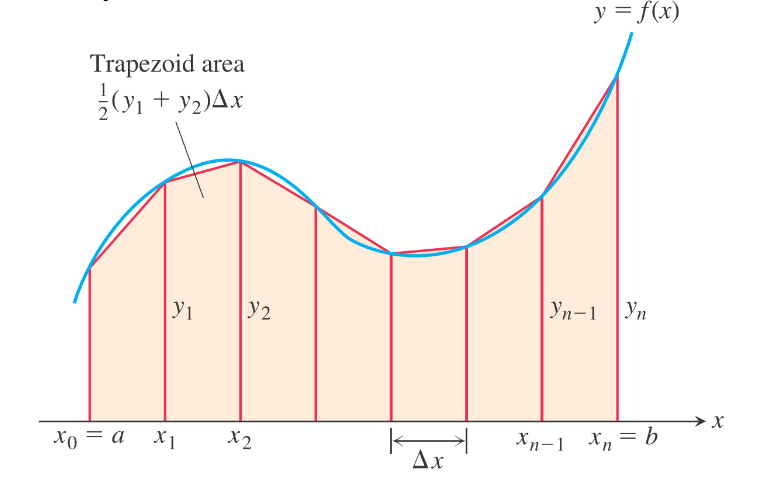
\includegraphics[width = 0.5\linewidth]{Images/trapezoid rule.png}
     \caption{Area of each partition is represented by a trapezoid}
\end{figure}
Instead of using $f(c_k)\Delta x_k$ in Riemann sum, we take 
\[
    T_k = \frac{(y_{k - 1} + y_k) \Delta x}{2} 
\]
where $y_k = f(x_k)$. $T_k$ is the area of a trapezoid if $f$ is non-negative.
\paragraph{Definition} For trapezoid rule, first let $P = \{x_0, x_1, ..., x_n\}$ be a partition of $[a, b]$, then  
\[
    \int_a^b f(x) \, dx \approx \sum_{k = 1}^n T_k = \frac{\Delta x}{2} (f(x_0) + 2f(x_1) + 2f(x_2) + \dots\, + 2f(x_{n - 1}) + f(x_n)) 
\]
where $\Delta x = \frac{b - a}{n}$

\subsection{Simpson's Rule}
In any Riemann Sum approximation $f$ is approximated by a \textbf{constant} $f(c_k)$ over the interval $[x_{k-1}, x_k]$.
In the Trapezoidal Rule, the function $f$ is approximated by a \textbf{linear function} $y = Ax + B$ over $[x_{k - 1}, x_k]$ whose
graph passes through the point $(x_{k-1}, y_{k - 1})$ and $(x_k, y_k)$

We can take this approach a step further by approximating $f$ with quadratic polynomials $Ax^2 + Bx + C$
\begin{figure}[H]
    \centering 
    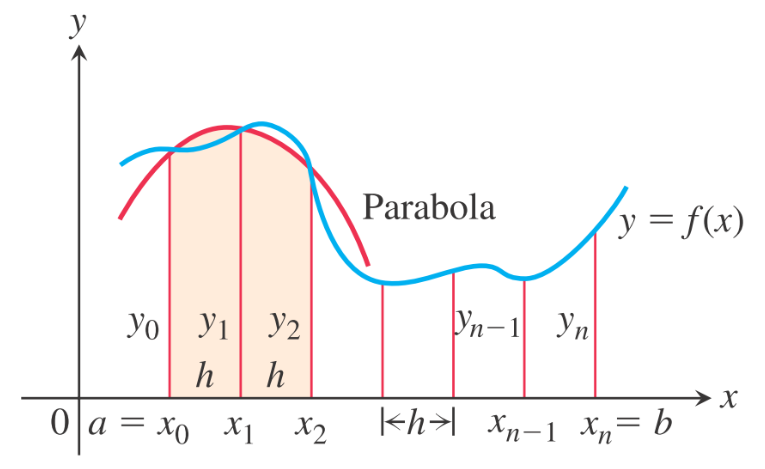
\includegraphics[width = 0.5\linewidth]{Images/simpson rule.png}
    \caption{Area of each partition is approximated by the area of \textbf{quadratic equation} passing three points}
\end{figure}

\noindent
Consider an evenly spaced partition $P = \{x_0, x_1, ..., x_n \}$ of $[a, b]$ where $n$ is even. For $k \in \{1,3,5,..., n-1\}$, over the interval $[x_{k - 1}, x_{k _ 1}]$ consider approximating $f$
by the quadratic function $p_k(x) = A_kx^2 + B_kx + C_k$ whose graph passes through the three points $(x_{k-1}, y_{k - 1})$, $(x_k, y_k)$ and $(x_{k+1}, y_{k + 1})$.
This approximation is called Simpson's Rule, that is
\[
    \int_a^b f(x) \, dx \approx \sum_{k \in \{1,3, \dots, n - 1 \}} \int_{x_{k - 1}}^{x_{k + 1}} p_k(x) \, dx
\]

First we consider $\int_{x_0}^{x_2} p_1 (x) \, dx$. We may shift the graph so that $x_0 = -\Delta x$, $x_1 = 0$, and $x_2 = \Delta x$ since shifting horizontally do not change
the valua of an integral, then we have 
\[
    \int_c^d f(x) \, dx = \int_{c - s}^{d - s} f(x) \, dx
\]
Let $h = \Delta x$, we write 
\[
    q_1(x) = Ax^2 + Bx + C = p_1(x + h + a)
\]
with $q_1(x)$ as shifted polynomial. Then 
\begin{align*} 
    \int_{x_0}^{x_2} p_1 (x) \, dx &= \int_a^{a + 2h} p_1(x) \, dx\, \\
    &= \int_{ - h}^{h} q_1(x) \, dx\, \\
    &= \int_{ - h}^{h} (Ax^2 + Bx + C) \, dx \\
    &= \left[\frac{A}{3}x^3 + \frac{B}{2}x^2 + Cx \right]^{h}_{ - h} \\
    &= 2\left(\frac{A}{3}h^3 + Ch \right) = \frac{h}{3} (2Ah^2 + 6C)
\end{align*}
Since $(-h, y_0), (0, y_1), (h, y_2)$ are all on the graph of $y = Ax^2 + Bx + C$, we have
\begin{align*} 
    y_0 &= Ah^2 - Bh + C \\
    y_1 &= C \\
    y_2 &= Ah^2 + Bh + C \\
    y_0 + y_2 &= 2Ah^2 + 2C = 2Ah^2 + 2y_1 \\
    2Ah^2 &= y_0 + y_2 - 2y_1 \\
\end{align*}
Hence, we have 
\[
    \int_{x_0}^{x_2} p_1(x) \, dx = \frac{h}{3} (2Ah^2 + 6C) = \frac{h}{3} (y_0 + 4y_1 + y_2)
\]
And generally:
\[
    \int_{x_{k - 1}}^{x_{k + 1}} p_k(x) \, dx = \frac{h}{3} (y_{k - 1} + 4y_{k} + y_{k + 1})
\]
Therefore:
\begin{align*} 
    \int_a^b f(x) \, dx &\approx \sum_{k \in \{1,3, \dots, n - 1 \} } \int_{x_{k - 1}}^{x_{k + 1}} p_k(x) \, dx\, \\
    &= \int_{x_0}^{x_2} p_1(x) \, dx + \int_{x_2}^{x_4} p_3(x) \, dx\, + \dots\, + \int_{x_{n - 2}}^{x_n} p_{n - 1}(x) \, dx\, \\
    &= \frac{h}{3} (y_0 + 4y_1 + 2y_2 + 4y_3 + 2y_4 + \dots\, + 2y_{n - 2} + 4y_{n - 1} + y_n)
\end{align*}
    
\paragraph{Definition} For Simpson's Rule, let $P = \{x_0, x_1, ..., x_n \}$ of $[a, b]$ where $n$ is even. For $k \in \{1,3,5,..., n-1\}$, then 
\[
    \int_a^b f(x) \, dx \approx \frac{\Delta x}{3} (y_0 + 4y_1 + 2y_2 + 4y_3 + 2y_4 + \dots\, + 2y_{n - 2} + 4y_{n - 1} + y_n)
\]
where $n$ is even and the coefficients are 1, 4, 2, 4, 2, 4, 2, ..., 4, 2, 4, 1
\subsection{Error Bounds}
Consider an example
\[
    I = \int_1^{1.6} \frac{1}{x} \, dx
\]
We will check the approximation using trapezoidal rule and simpson's rule using $\Delta x = 0.1$ 

\paragraph{Trapezoidal Rule}
\[
    I \approx \frac{0.1}{2} (\frac{1}{1} + \frac{2}{1.1} + \frac{2}{1.2} + \dots\, + \frac{2}{1.5} + \frac{1}{1.6}) \approx 0.470510739
\]

\paragraph{Simpson Rule}
\[
    I \approx \frac{0.1}{3} (\frac{1}{1} + \frac{4}{1.1} + \frac{2}{1.2} + \dots\, + \frac{4}{1.5} + \frac{1}{1.6}) \approx 0.470064
\]
Using FTC to solve the integration we get 
\[
    I = \int_1^{1.6} \frac{1}{x} \, dx = \ln 1.6 - \ln 1 = \ln 1.6 = 0.470003629
\]
Hence for this example we have
\[
    |E_S| < |E_M| < |E_T| < |E_R| < |E_L|
\]
with $L$ as left-hand Riemann sum, $R$ as right-hand Riemann sum, $M$ as midpoint Riemann sum, $T$ as Trapezoidal rule and $S$ as Simpson's rule.

\noindent
Let $f$ be a function that is integrable on $[a, b]$, and let 
\[
    \max |f^{(i)}| = \max_{x \in [a, b]} |f^{(i)}(x)|
\]
then we have error bounds for each approximation:
\begin{align*} 
   &|E_L| \leq \frac{(b - a)^2}{2n} \max |f'| \textrm{\tab}  &|E_R| \leq \frac{(b - a)^2}{2n} \max |f'|\, \\
   &|E_T| \leq \frac{(b - a)^3}{12n^2} \max |f''| \textrm{\tab}  &|E_M| \leq \frac{(b - a)^3}{24n^2} \max |f''|\,
\end{align*}
\[
    |E_S| \leq \frac{(b - a)^5}{180n^4} \max |f^{(4)}| 
\]

\paragraph{Example} If we want to approximate 
\[
    \int_0^1 e^{x^2} \, dx
\]
with $|E| < 10^{-5}$, how many sub intervals do we need at least for the trapezoidal rule and Simpson's rule?
Let $f(x) = e^{x^2}$ then  
\begin{align*} 
     f'(x) &= ex^2 2x \\
     f''(x) &= e^{x^2}(4x^2 + 2) < 6e \\
     f'''(x) &= e^{x^2}(8x^3 + 12x) < 20e \\
     f^{(4)}(x) &= e^{x^2}(16x^4 + 48x^2 + 12) < 76e 
\end{align*}
For Simpson's rule:
\begin{align*} 
    |E_S| \leq \frac{1}{180n^4} 76e < 10^{ - 5}
    n^4 > \frac{76e \times 10^5}{180} = 19 
\end{align*}
For the trapezoidal rule:\begin{align*} 
    |E_S| \leq \frac{1}{12n^2} 6e < 10^{ - 5}
    n^4 > \frac{6e \times 10^5}{12} = 369 
\end{align*}

\paragraph{Remarks} To determine whether the riemman sum is an overestimate or underestimate, we can see from:
\begin{itemize} 
     \item For an \textbf{increasing curve}, left-side sum is an underestimate and the right-side sum is an overestimate
     \item For a \textbf{decreasing curve}, left-side sum is an overestimate and the right-side sum is an underestimate
     \item For a \textbf{concave up curve}, trapezoidal rule is an overestimate and the mid-point sum is an underestimate
     \item For a \textbf{concave down curve}, trapezoidal rule is an underestimate and the mid-point sum is an overestimate
     \item Simpson's rule gives an exact answer for polynomials with degree lower than four (because the fourth derivative is 0, then the error = 0)
\end{itemize}
\section{Improper Integrals}
\subsection{Improper Integrals Type 1}
\begin{figure}[H]
     \centering
     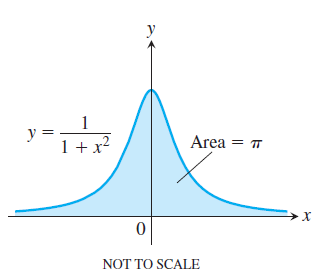
\includegraphics[width = 0.5\linewidth]{Images/improper type 1.png}
\end{figure}
\paragraph{Definition} Integrals with infinite limites of integrations are improper integrals type 1:
\begin{enumerate} 
     \item Let $a \in \mathbb{R}$. If $f$ is integrable on $[a, b]$ for every $b \in [a, \infty)$ then 
     \[
         \int_a^{\infty} f(x) \, dx = \lim_{b \to \infty} \int_a^b f(x) \, dx
     \]
     \item Let $b \in \mathbb{R}$. If $f$ is integrable on $[a, b]$ for every $a \in (-\infty, b]$ then 
     \[
         \int_{ -\infty}^{b} f(x) \, dx = \lim_{a \to - \infty} \int_a^b f(x) \, dx
     \]
     \item If $f$ is integrable on $(- \infty, \infty)$, and let $c \in \mathbb{R}$ then
     \[
        \int_{ -\infty}^{\infty } f(x) \, dx = \int_{ -\infty}^{c} f(x) \, dx + \int_{c}^{\infty } f(x) \, dx
     \]
\end{enumerate}

\paragraph{Definition: Convergence} An improper integral is said to be convergent if the corresponding limit exists, and is said to be divergent if the limit does not exist as real number.

\paragraph{Remarks} The definition (3) also applies to the case where we have $\infty + \infty$, $-\infty - \infty$ or $a \pm \infty$ on the right, but it is not defined if either 
the right hand side is an indeterminate form (e.g., $\infty - \infty$) or one of the terms on the right does not exist. \\

\noindent
If the function $f$ is always positive in the interval of integration, then the improper integrals can be viewed as the area between the graph and the x-axis.

\paragraph{Example 1} Find 
\[
    \int_1^{\infty} \frac{1}{x} \, dx
\] 

\begin{align*} 
    \int_1^{\infty} \frac{1}{x} \, dx &= \lim_{b \to \infty} \int_1^b x\frac{1}{x} \, dx \\
    &= \lim_{b \to \infty} \ln |b| - \ln |1| = \ln |b| \\
    &= \infty \textrm{\tab diverge}
\end{align*}
\paragraph{Example 2} For $\alpha \neq 1$, find 
\[
    \int_1^{\infty} x^{\alpha} \, dx
\]
\begin{align*} 
    \int_1^{\infty} x^{\alpha} \, dx &= \lim_{b \to \infty} \int_1^{b} x^{\alpha} \, dx \\
    &= \lim_{b \to \infty} \frac{1}{\alpha + 1} (b^{\alpha + 1} - 1) \\
    &= \begin{cases} 
        \infty & \alpha > - 1 \\
        - \frac{1}{\alpha + 1} & \alpha < - 1
    \end{cases} 
\end{align*}
\paragraph{Example 3} Find
\[
    \int_{ -\infty}^{\infty} \frac{1}{1 + x^2} \, dx
\]
\begin{align*} 
    \int_{ -\infty}^{\infty} \frac{1}{1 + x^2} \, dx &= \lim_{b \to \infty} \int_{0}^{b} \frac{1}{1 + x^2} \, dx\, + \lim_{a \to - \infty} \int_{a}^{0} \frac{1}{1 + x^2} \, dx \\
    &= \lim_{b \to \infty} \arctan b - \arctan 0 + \lim_{a \to \infty} \arctan 0 - \arctan a \\
    &= \lim_{b \to \infty} \arctan\, b\, - \lim_{a \to \infty} \arctan  a \\
    &= \frac{\pi}{2} + \frac{\pi}{2} = \pi
\end{align*}

\subsection{Improper Integrals Type 2: Dicontinuity}
\begin{figure}[H]
    \centering
    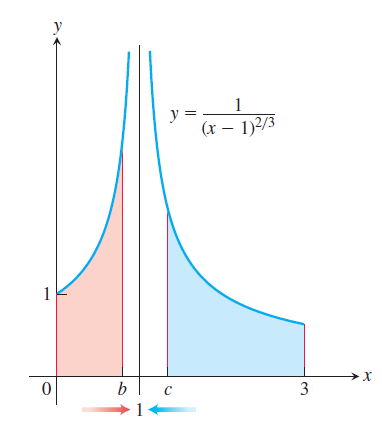
\includegraphics[width = 0.35\linewidth]{Images/improper type 2.png}
\end{figure}
\paragraph{Definition}
If $f$ is continuous on $[a, b)$ and is discontinuous at $b$ then 
\[
    \int_a^b f(x) \, dx = \lim_{c \to b^{ - }} \int_a^c f(x) \, dx
\]
If $f$ is continuous on $(a, b]$ and is discontinuous at $a$ then 
\[
    \int_a^b f(x) \, dx = \lim_{c \to a^{ + }} \int_c^b f(x) \, dx
\]
If $f$ i discontinuous at $c$ where $a < c < b$ and is continuous on $[a, b] \setminus\{c\}$
\[
    \int_a^b f(x) \, dx = \int_a^c f(x) \, dx +\int_c^b f(x) \, dx
\]

The definition above is defined if the right hand side is $\infty + \infty$, $- \infty - \infty$ and $a \pm \infty$
but is not defined if the right hand side is $\infty - \infty$

\paragraph{Example 1} Suppose $p > 0$
\[
    \int_0^1 \frac{1}{x^p} \, dx
\]
Since 
\[
    \lim_{x \to 0^{ +}} \frac{1}{x^p} = \infty
\]
It has essential discontinuity at $x = 0$

\begin{align*} 
     \int_a^1 \frac{1}{x^p} \, dx &= \left[\frac{1}{ - p + 1} x^{ - p +1} \right]_a^1 \textrm{\tab } p \neq 1 \\
    &= \frac{1}{1 - p}(1 - \frac{1}{a^{p - 1}}) \\
    &= \begin{cases} 
        \infty & p > 1 \\
        \frac{1}{1 - p} & 0 < p < 1
    \end{cases} 
\end{align*}
If $p = 1$
\begin{align*} 
    \int_0^1 \frac{1}{x} \, dx\, = \lim_{a \to 0^+} (\ln 1 - \ln a) = \infty
\end{align*}
Hence
\begin{align*} 
    \int_0^1 \frac{1}{x^p} \, dx \begin{cases} 
        \textrm{converges to  } \frac{1}{1 - p} & 0 < p <1 \\
        \textrm{diverges to } \infty & p \geq 1
    \end{cases} 
\end{align*}
Combined with type 1 improper integrals we now know the convergence of $\int_0^{\infty} \frac{1}{x^p}$:
\begin{itemize} 
    \item If $0 < p < 1$: $\int_0^1 \frac{1}{x^p} \, dx$ converges, and $\int_1^{\infty} \frac{1}{x^p} \, dx$ diverges.
    \item If $p > 1$: $\int_0^1 \frac{1}{x^p} \, dx$ diverges, and $\int_1^{\infty} \frac{1}{x^p} \, dx$ converges.
    \item If $p = 1$: Both $\int_0^1 \frac{1}{x^p} \, dx$ and $\int_1^{\infty} \frac{1}{x^p} \, dx$ diverges.
\end{itemize}

\paragraph{Example 2} Find
\[
    \int_0^3 \frac{1}{x - 1} \, dx 
\]

Note that $\frac{1}{x-1}$ is continuous on $[0, 3] \setminus \{1\}$.
\begin{align*} 
     \int_0^1 \frac{1}{x - 1} \, dx = \lim_{a \to 1^{ -}} (\ln |a - 1| - \ln |- 1|) = - \infty \\
     \int_1^3 \frac{1}{x - 1} \, dx = \lim_{a \to 1^{ +}} (\ln |3 - 1| - \ln |a - 1|) = \infty \\
\end{align*}
Hence
\[
    \int_0^3 \frac{1}{x - 1} \, dx\, = \infty - \infty 
\]
which is by definition undefined
\subsection{Convergence Test}
For some integral of function that has no elementary antiderivative, such as $e^{x^2}$, numerical method is required. To
find the convergence, convergence test is needed.

\begin{theorem}[Direct Comparison Test]
    Suppose that $a \in \mathbb{R}$ and suppose that $f$ and $g$ are continuous functions on $[a, \infty)$. If there exists $c \in [a, \infty)$ such
    that $0 \leq f(x) \leq g(x)$ for all $x \in [c, \infty)$ then the following statements hold:
    \begin{enumerate}[i]
        \item If $\int_a^{\infty} g(x) \, dx$ converges, then $\int_a^{\infty} f(x) \, dx$ converges.
        \item If $\int_a^{\infty} f(x) \, dx$ diverges, then $\int_a^{\infty} g(x) \, dx$ diverges.
    \end{enumerate}
\end{theorem}

\paragraph{Intuition Proof (i)}
Since $\int_a^{\infty} g(x) \, dx = \int_a^c g(x) \, dx + \int_c^{\infty} g(x) \, dx$ then $\int_a^{\infty} g(x) \, dx$ converges if and only if $\int_c^{\infty} g(x) \, dx$ converges.
This also holds for $f(x)$. Hence it suffices to show that if $\int_c^{\infty} g(x) \, dx$ converges then $\int_c^{\infty} f(x) \, dx$ converges.
By domination rule of definite integral for all $x \in [c, \infty)$ we have
\[
    0 \leq \int_c^t f(x) \, dx \leq \int_c^t g(x) \, dx
\]
Assume that $\int_c^{\infty} g(x) \, dx$ converges then for some $L \in \infty$ 
\[
    \lim_{t \to \infty} \int_c^t g(x) \, dx = L
\]
Hence, $\int_c^t f(x) \, dx$ is bounded above by $L$ and has a least upper bound, for example, $A$.
Then 
\[
    \lim_{t \to \infty} \int_c^t f(x) \, dx = \int_c^{\infty} f(x) \, dx = A
\]

\paragraph{Example 1} Determine the convergence of 
\[
    \int_0^{\infty} e^{ - x^2} \, dx
\]

For all $x \in [1, \infty)$ we have $x^2 \geq x > 0$, we have
\[
    e^{x^2} \geq e^{x} > 0 \Rightarrow 0 < e^{ - x^2} \leq e^{ - x} \textrm{\tab} \forall \, x \in [1, \infty)
\]

Since
\[
    \int_0^{\infty} e^{ - x} \, dx = \lim_{b \to \infty} ( - e^{ - b} + e^{ - 0}) = 1 \textrm{  (converges)}
\]
then by direct comparison test, $\int_0^{\infty} e^{-x^2} \, dx$ also converges.

\paragraph{Example 2} Determine the convergence of 
\[
    I = \int_2^{\infty} \frac{\sqrt[3]{x^7 + 2}}{x^3 \ln x} \, dx 
\]

\[
    \frac{\sqrt[3]{x^7 + 2}}{x^3 \ln x}\, \approx \frac{x^{\frac{7}{3}}}{x^2 x \ln x} = \frac{x^{\frac{1}{3}}}{x \ln x} > \frac{1}{x \ln x} > 0 \textrm{\tab} \forall \, x > 1
\]

Then try comparison test with $\int_2^{\infty} \frac{1}{x \ln x} \, dx$, let $u = \ln x$:
\begin{align*} 
    \int_2^{\infty} \frac{1}{x \ln x} \, dx = \lim_{b \to \infty} \int_{\ln 2}^{\ln b} \frac{du}{u} \\
    &= \lim_{b \to \infty} [\ln (u)]_{\ln 2}^{\ln b} \\
    &= \lim_{b \to \infty} (\ln(\ln b) - \ln(\ln 2)) = \infty
\end{align*}

Since $\int_2^{\infty} \frac{1}{x \ln x} \, dx$ diverges, then by comparison test $I$ also diverges

\begin{theorem}[Limit Comparison Test]
     Suppose that $a \in \mathbb{R}$ and suppose that $f$ and $g$ are positive continuous functions on $[a, \infty)$. If 
     \[
         \lim_{x \to \infty} \frac{f(x)}{g(x)} = L 
     \]
     for some $L \in \mathbb{R_{+}}$ then 
     \[
         \int_a^{\infty} f(x) \, dx \textrm{\tab and \tab} \int_a^{\infty} g(x) \, dx
     \]
     both converge or both diverge
\end{theorem}

\paragraph{Proof}
Since $\lim_{x \to \infty} \frac{f(x)}{g(x)} = L$, $\exists \, M \in \mathbb{R} : \forall \, x \in [M, \infty)$
\[
    \frac{L}{2} \leq \frac{f(x)}{g(x)} \leq \frac{3L}{2} \Rightarrow 0 < \frac{L}{2} g(x) \leq f(x) \leq \frac{3L}{2} g(x)
\]
If $\int_a^{\infty} f(x) \, dx$ converges then $\int_a^{\infty} \frac{L}{2} g(x) \, dx$ converges so
\[
    \int_a^{\infty} g(x) \, dx = \frac{2}{L} \int_a^{\infty} \frac{L}{2} g(x) \, dx 
\]
also converges.

\noindent
If $\int_a^{\infty} f(x) \, dx$ diverges then $\int_a^{\infty} \frac{3L}{2} g(x) \, dx$ diverges so
\[
    \int_a^{\infty} g(x) \, dx = \frac{2}{3L} \int_a^{\infty} \frac{3L}{2} g(x) \, dx 
\]
also diverges.

\paragraph{Example} Find the convergence of 
\[
    I = \int_1^{\infty} \frac{1 - e^{ - x}}{x} \, dx 
\]
(1) Using direct comparison test:
\[
    0 < \frac{1 - e^{ - x}}{x} < \frac{1}{x} 
\]
Despite we know that $\int_1^{\infty} \frac{1}{x} \, dx$ diverges, the convergence of $I$ can not be known by direct comparison test. \\
(2) Limit comparison test
\[
    \lim_{x \to \infty} \frac{\frac{1 - e^{ - x}}{x}}{\frac{1}{x}} = \lim_{x \to \infty} (1 - e^{ - x}) = 1
\]
By limit comparison test, since $\int_1^{\infty} 1/x \, dx$ diverges, $I$ also diverges.

\paragraph{Remarks}
If $f$ and $g$ are positive and continuous on $[a, \infty)$ and $\lim_{x \to \infty} \frac{f(x)}{g(x)} = L$ then
\begin{itemize} 
    \item If $L = 0$ and $\int_a^{\infty} g(x) \, dx$ converges then $\int_a^{\infty} f(x) \, dx$ converges 
    \item If $L = \infty$ and $\int_a^{\infty} g(x) \, dx$ diverges then $\int_a^{\infty} f(x) \, dx$ diverges 
\end{itemize}
\end{document}
